%!TEX TS-options = --shell-escape
% CfAI Thesis template - prepared by Matthew Townson and Andrew Reeves, 2016

\documentclass[11pt, oneside, a4paper]{memoir}

% Packages for use in the thsis
\usepackage[utf8]{inputenc}
\usepackage[T1]{fontenc}
\usepackage{lmodern}
\usepackage[a4paper,width=138mm,top=35mm,bottom=35mm,bindingoffset=10mm]{geometry}
\usepackage{url}
\usepackage{titlesec}
\usepackage{graphicx}
\usepackage{hyperref}
\usepackage{rotating}
\usepackage{listings}
% \usepackage{gensymb}
\usepackage{pdflscape}
\usepackage{mathrsfs,amsmath}
\usepackage{units}
\usepackage{siunitx}
\usepackage{acronym}
\usepackage{booktabs}
\usepackage[UKenglish]{babel}
\usepackage{bibentry}
\usepackage{subcaption}
\usepackage{natbib}
\usepackage[export]{adjustbox}
% Bibliography Style

\bibliographystyle{abbrvnat}
\setcitestyle{authoryear,open={(},close={)}}
\usepackage{perpage}
\MakePerPage{footnote}
% \usepackage{minted}

\captionsetup[subfigure]{labelformat=simple}
\renewcommand\thesubfigure{\alph{subfigure})}


% Skip a line for new paragraph instead of indenting
\setlength{\parindent}{0pt}
\nonzeroparskip

\newsubfloat{figure}


%Define some useful aliases
\newcommand{\thesisTitle}{Exploitation}
\newcommand{\thesisSubtitle}{More like CTFs}
\newcommand{\thesisName}{Kalp Shah}
\newcommand{\thesisDate}{\today}
\newcommand{\thesisFirstSupervisor}{}
%\newcommand{\thesisSecondSupervisor}{Second Supervisor}
\newcommand{\thesisUniversity}{\protect{IIIT Hyderabad}}
%\newcommand{\thesisUniversityDepartment}{Department of Physics}
%\newcommand{\thesisUniversityInstitute}{Centre for Advanced Instrumentation}
\newcommand{\thesisUniversityCity}{Hyderabad}
%\newcommand{\thesisUniversityStreetAddress}{South Road}
%\newcommand{\thesisUniversityPostalCode}{DH1 3LE}


%to prefix appendix names with "Appendix"
\renewcommand*{\cftappendixname}{Appendix\space}

\renewcommand{\thefootnote}{\fnsymbol{footnote}}



\chapterstyle{madsen}



% Choice of line spacing (both valid)
% \OnehalfSpacing
\DoubleSpacing


\setsecnumdepth{subsection}


\nobibliography*


% Modify Headers
\makepagestyle{myruled}
\makeheadrule {myruled}{\textwidth}{\normalrulethickness}
\makefootrule {myruled}{\textwidth}{\normalrulethickness}{\footruleskip}
\makeevenhead {myruled}{}{\small\itshape\leftmark}{}
\makeoddhead {myruled}{}{\small\itshape\rightmark}{}
\makeevenfoot {myruled}{\small \thepage}{}{}
\makeoddfoot {myruled}{}{}{\small \thepage}

\makepsmarks {myruled}{
\nouppercaseheads
\createmark {chapter} {both} {shownumber}{}{. \ }
\createmark {section} {both}{shownumber}{} {. \ }
\createmark {subsection} {both}{shownumber}{} {. \ }
\createmark {subsubsection}{both}{shownumber}{} {. \ }
\createplainmark {toc} {both} {\texsname}
\createplainmark {lof} {both} {\listfigurename}
\createplainmark {lot} {both} {\listtablename}
\createplainmark {bib} {both} {\bibname}
\createplainmark {index} {both} {\indexname}
\createplainmark {glossary} {both} {\glossaryname}
}

\makepagestyle{plain}
\makefootrule {plain}{\textwidth}{\normalrulethickness}{\footruleskip}
\makeevenfoot {plain}{\small \thepage}{}{}
\makeoddfoot {plain}{}{}{\small \thepage}

\makepsmarks {plain}{
\nouppercaseheads
\createmark {chapter} {both} {shownumber}{}{. \ }
\createmark {section} {both}{shownumber}{} {. \ }
\createmark {subsection} {both}{shownumber}{} {. \ }
\createmark {subsubsection}{both}{shownumber}{} {. \ }
\createplainmark {toc} {both} {\texsname}
\createplainmark {lof} {both} {\listfigurename}
\createplainmark {lot} {both} {\listtablename}
\createplainmark {bib} {both} {\bibname}
\createplainmark {index} {both} {\indexname}
\createplainmark {glossary} {both} {\glossaryname}
}


\setsecnumdepth{subsubsection}
\pagestyle{myruled}


\begin{document}
\frontmatter
% !TEX root = ../thesis.tex
% --------------------------
% Front matter
% --------------------------
\pagenumbering{roman}           % roman page numbing (invisible for empty page style)
\pagestyle{empty}               % no header or footers
% !TEX root = ../thesis.tex

\begin{titlingpage}
    \begin{center}
        \vspace*{1cm}

        \Huge
        \textbf{\thesisTitle{}}

        % \Large
        \vspace{0.5cm}
        % \thesisSubtitle{}

        \vspace{1.5cm}

        
\includegraphics[width = 0.4\textwidth]{gfx/logo.png}

        \vfill

        \large

        \vspace{0.8cm}


        IIIT Hyderabad\\
        India\\
        December '19
        % \today

    \end{center}
\end{titlingpage}
      % INCLUDE: all titlepages
\cleardoublepage

\pagestyle{plain}               % display just page numbers
% !TEX root = ../thesis.tex
%
\hfill
\begin{center}
%\textbf{{\Large \thesisTitle}}\\
%\textbf{{\large \thesisName}}\\
\end{center}

\begin{abstract}
A thorough foray into exploitation and explanation of why it 
works the way it does. It is a compilation of sorts, and hence no 
correlation between chapters ( No flow b/w chapters exist ) and the 
book should exist as a case study and used to solve problems which 
look similar and also has some basics which I go learning on the 
way forward.

\end{abstract}

\vfill
    % \thesisDate \\
    % Reviewers: \thesisFirstReviewer\ and \thesisSecondReviewer \\
    % \textbf{\thesisUniversity} \\
    % \textit{\thesisUniversityGroup} \\
    % \thesisUniversityInstitute \\
    % \thesisUniversityDepartment \\
    % \thesisUniversityStreetAddress \\
    % \thesisUniversityCity \\
    % \thesisUniversityPostalCode
        % INCLUDE: the abstracts (english and german)
\cleardoublepage
%
% !TEX root = ../thesis.tex
%
% \pdfbookmark[0]{Acknowledgement}{Acknowledgement}
\chapter*{Sources}
\label{sec:acknowledgement}
% \vspace*{-10mm}
\begin{OnehalfSpacing}
The websites and competitions referred for writing this piece :
\begin{itemize}
    \item \href{https://ctf101.org}{CTF 101}
    \item \href{https://shellterlabs.com}{Shellter Labs}
    \item Linux Man Pages
    \item \href{https://picoctf.com}{picoCTF}
    \item \href{https://trailofbits.github.io/ctf}{trailofbits}
    \item \href{http://www.cs.fsu.edu/~redwood/OffensiveComputerSecurity/lectures.html}{Florida University Computer Security}
    \item \href{https://www.megabeets.net/a-journey-into-radare-2-part-1/}{Megabeets Radare Tutorial}
    \item \href{https://developer.android.com/studio/command-line/adb}{Android Developers Website}
\end{itemize}    
\end{OnehalfSpacing}
 % INCLUDE: acknowledgement
\cleardoublepage
%
\setcounter{tocdepth}{3}        % define depth of toc
\cleardoublepage
%
% !TEX root = ../thesis.tex
%
%************************************************
% Declaration
%************************************************
% \pdfbookmark[0]{Declaration}{Declaration}

\chapter{Declaration}
\label{sec:declaration}
\begin{OnehalfSpacing}
This is just to explain how certain exploits work in a great detail.

%\section*{Publications}
%Relevant Publications

% \bigskip
%
% \noindent\textit{\thesisDate}
%
% \smallskip
%
% \begin{flushright}
%     \begin{minipage}{5cm}
%         \rule{\textwidth}{1pt}
%         \centering\thesisName
%     \end{minipage}
% \end{flushright}

\vfill

    ``\emph{If it moves, compile it}''.

\end{OnehalfSpacing}

%*****************************************
%*****************************************

\cleardoublepage
%
%\listoffigures
\cleardoublepage
%
%\listoftables
\cleardoublepage


\newpage

% !TEX root = ../thesis.tex
% \pdfbookmark[0]{Acronyms}{Acronyms}
\chapter{Basics}
\section{Data}
There are many places to store data on a typical computer like 
a hard drive ( or any other secondary storage ), RAM, Caches 
and Registers.\\\\A hierarchy is decided on their access speed. 
If a piece of data is required more frequently, it is stored on 
a faster storage device. ( Faster implies lower latency i.e. time 
taken from being asked for data and providing it ). The figure 1 
shows this heirarchy.\\

\begin{figure}
    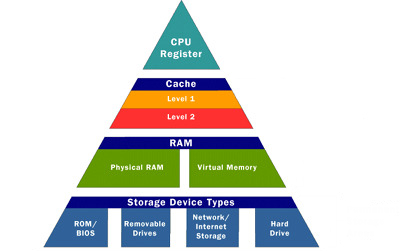
\includegraphics[width = 0.50\textwidth, center]{gfx/storageHierarchy.jpg}    
    \caption{Latency Hierarchy}
\end{figure}

\subsection*{Location}

\subsubsection*{Register}
A register is located in the CPU itself and as it is physically the
closest, it also the fastest. It is the one that is accessed while
running a program\\\\ A sample data flow can be seen in Figure 2, which shows
data tranfer from RAM to Register and then to the CPU.

\begin{figure}
    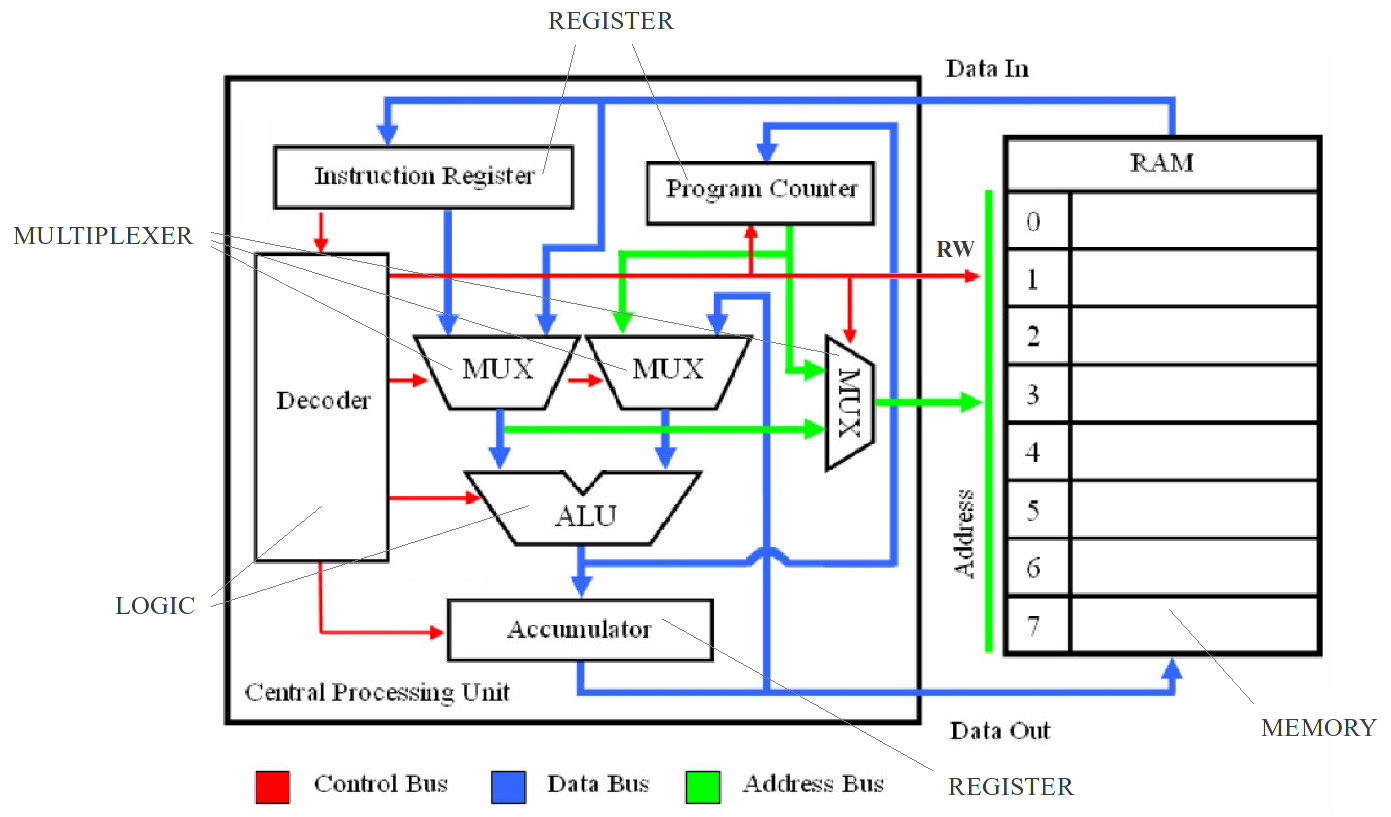
\includegraphics[width = 0.9\textwidth, center]{gfx/cpu.jpg}    
    \caption{Circuit of CPU}
\end{figure}

\subsubsection*{Cache}
A cache is small piece of memory located near the CPU and works as a
faster RAM (sort of). It caches the data which the OS thinks is required 
the most.\\\\L1 \& L2 cache is built into the proccessor (recent ones anyway) 
and is individual for every physical core whereas L3 cache is located
outside of the actual silicon but is in the chip and so is common for 
all cores.

\subsubsection*{RAM}
RAM is a volatile memory where all the memory that is deemed by the 
OS as required is stored for instant access with the CPU. The data 
tranfer happens from RAM $\rightarrow$ Cache $\rightarrow$ Register.

\subsection*{Bridges}
Bridges are small microcontrollers with built in logic which help in 
communication with external devices. There are two of there, and are 
descibed by their position on the board and also the threshold speed 
they can manage.
\subsubsection*{North Bridge}
 North bridge is a controller chip which connect high speed external 
 devices to the chipset. It was originaly outside ot the main chip 
 and an external silicon but now is mostly included in the SoC ( System on
 a chip ). The devices which can be connected to it are given in 
 Figure 3.

 \begin{figure}
    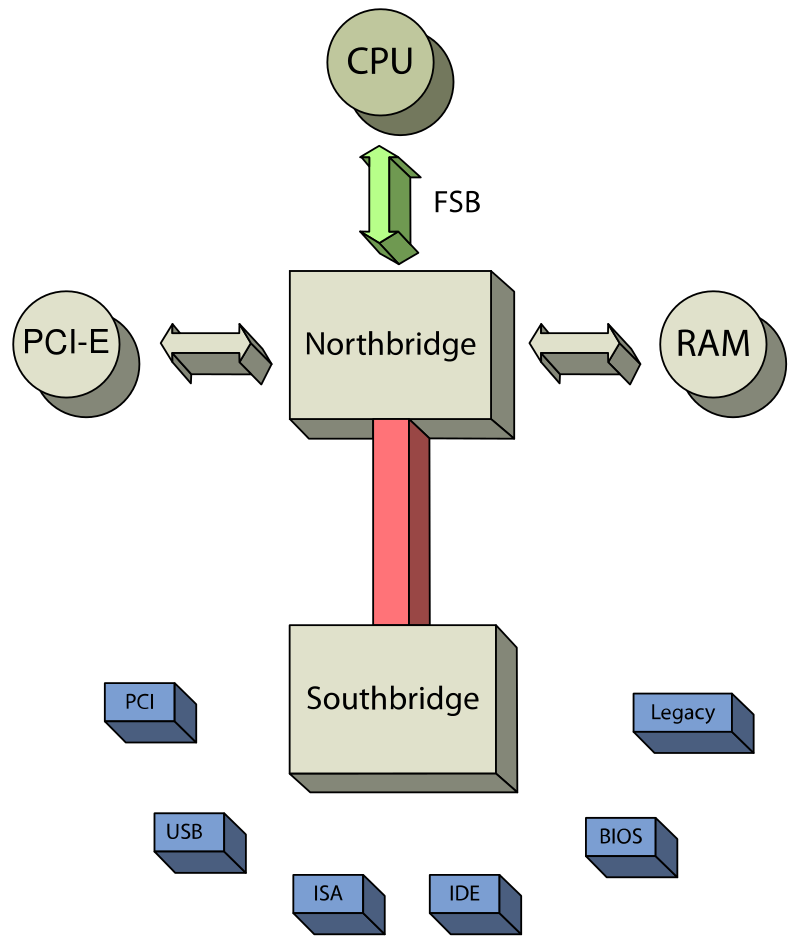
\includegraphics[width = 0.50\textwidth, center]{gfx/ChipSchem.png}    
    \caption{Use of bridges}
\end{figure}

\begin{figure}
    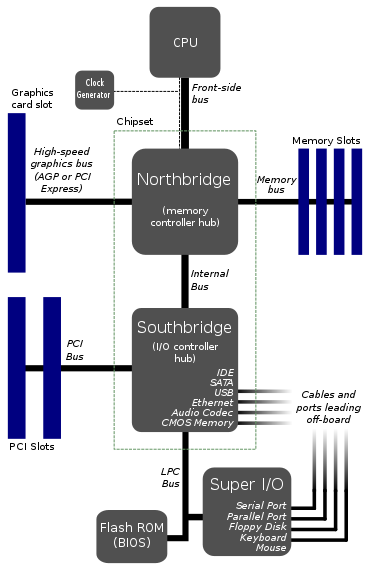
\includegraphics[width = 0.50\textwidth, center]{gfx/Motherboard.png}    
    \caption{Schematic Design of Bridges}
\end{figure}

\subsubsection*{South Bridge}
South bridge is the chipset which connects slower and legacy devices 
to the main chip. It is still seperate on Intel boards but is now 
starting to get integrated in AMD motherboards.

\subsection*{Data Flow}
So the data flow happens as follows :
\begin{center}$Solid\ State \rightarrow South\ Bridge \rightarrow RAM 
\rightarrow Register $
\end{center}
So when a computer is started, it first POSTS and then goes to 
the BIOS after which the BIOS piont the program to the Magic Number 
( For legacy MBR systems ) which has the bootloader in it (Like GRUB), 
after which the bootloader takes control of the System, then loades the 
kernel and with that the OS, which loads itself in the RAM, for fast 
access (The most recently executed programs still in the registers and 
cache) after which the OS loads a GUI ( If it has one ) or just greets 
to a TTY terminal. For the non GUI version, it gets you to a log in 
screen, whicle for GUI an application is loaded which takes care of 
logging in ( Known as a Display Manager (DM) ).

\begin{figure}
    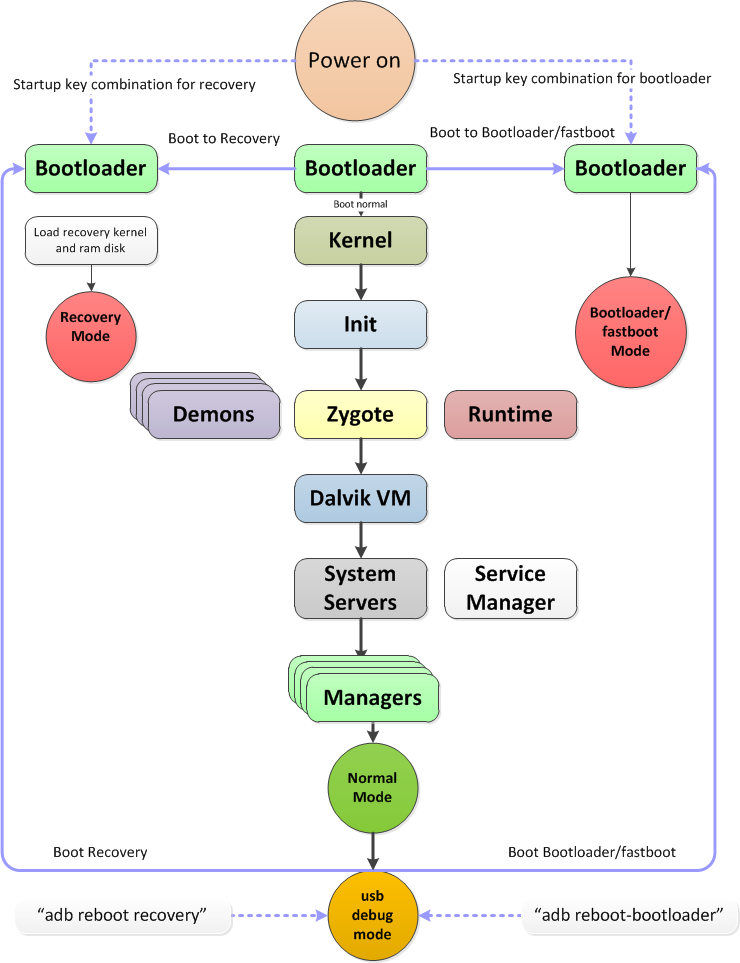
\includegraphics[width = 0.60\textwidth, center]{gfx/android-booting-process.png}    
    \caption{Android booting process}
\end{figure}

% !TEX root = ../thesis.tex
% \pdfbookmark[0]{Acronyms}{Acronyms}
\chapter{Tools}
There are many tools which make analysing and understaing flaws of programs very easy. Most of them are not required and work can be done without them, but they are a good creature comfort and sholud be used as such. These tools are used to analyse a piece of code and understand its vulnerabilites and also to  generate payloads to make exploiting them easier.

\section{GDB}
GDB is one of the most importatnt tools. It is one of, if not the most importatnt tool for exploiting binaries. It is essentially a debugger which allows for dissasmbly of binaries, is also usefull for checking the flow of the the binary, and before Ghidra was one of the most popular tools to understand the working of a program. It is still used for basic analysis, to check if the exploit works, and for initial routing checking. If someone is starting out with binary exploitation, then that someone should exclusively use GDB till the fundamentals of exploitation done are understood.

\subsection*{Basic Setup}
GDB is usually pre installed on any linux machine. But if it isn't, it can be installed using the default package manager ( Like apt or pacman ). There are some extensions for GDB that make it a much easier tool to operate with. You can use any number of them to make it to your liking, but in the following section, only some extensions are used and explained.

\section{radare2}
Radare is a tool which helps in understanding the binary, decompiling 
it and allowing to modify commands on the fly. It is considered one of 
the most difficult tools to master, so much so, that they themselves 
put Figure 6 on their website. I think this can be the Maya of exploiation 
tools.

\begin{figure}
    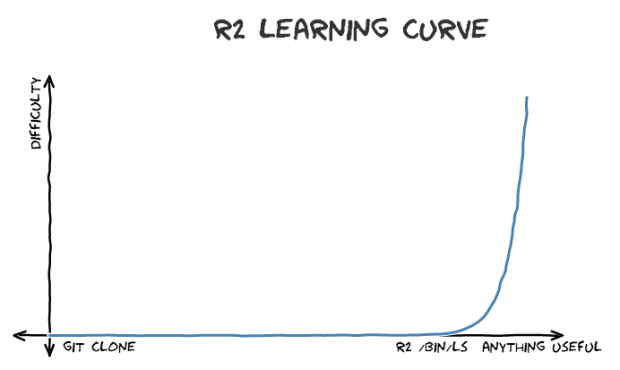
\includegraphics[width = 0.50\textwidth, center]{gfx/radare_learning.png}    
    \caption{Radare Learning Curve}
\end{figure}

\mainmatter

\pagestyle{myruled}

%%%%%%%%%%%%%%%%%%%%%%%%%%%%%%%%%
% Include your chapters here!
\setcounter{equation}{0}

\chapter{Binary Exploits}

\section*{Introduction}
Binary exploitation is the process of subverting a compiled application
t it violates some trust boundary in a way that is advantageous to you, 
the attacker.The exploits are explained breifly and then given case 
studies for it to be understood better.

\section{Buffer Overflow}
A buffer overflow occurs when a piece of data overflows the storage space
given to it. In these types of exploits, usually stack smashing occurs which 
changes value of non intended variables and helps in changing the flow of the 
program in some way.

\subsection{Stack}
One of the most important component to understand for binary exploitation and 
by extention buffer overflow is the stack. It is the location where all the 
variables and  % INCLUDE: introduction
\setcounter{equation}{0}

\chapter{Systems and Exploitation}

\section*{Introduction}
The following chapter is an introduction to case studies of well knowns exploits, 
intoducing mobile systems and gaming consoles ( The easiest 
to hack, for their exploitation is mainstream ). This is an introduction 
to the basics of actual life exploiting and will go into details 
on how the exploits were used, how to install them, their working 
and also how to replicate it.\\\\Specific systems will be covered 
in a one to one case based scenario. 

\section*{Terminology}
There are some very common terms encountered while browsing through 
this piece and also while refering to external resources specific 
to console exploitation ( As I told you, it \textit{was} (is) very mainstream )
\\\\Exploitation of systems with only a software is known as a 
softmod, whereas one done by physically modifying your hardware 
is known as hardmod. There are obvious advantages to both, a softmod 
is usually protected from in the next firmware update whereas hardmods 
are usually based on hardware vulnerabilities ( But not always ) and 
thus are harder to protect against after product is in the hands of 
the public.

\section{PSP}
One of the most exploited ( \textit{Hacked} ) system out there. It is the 
one that even I have reaped the benifits of, by doing \textit{legal} things, 
of course. It is also the one which I remember following to check 
out if the next version was exploitable, was it safe, did the risks 
outweigh the positives, etc. So here, I will explain how the PSP 
was exploited, why was it \textit{easy} and also replication.

\section{Android}
For android devices, it is not technically exploitaion as Android 
does not dissalow it, it is the OEMs which refuse access to root 
for customers. So rooting \textit{technically}, if the OEM ( like 
Xiaomi ) allows it, is not exploitaiton, but it does allow 
access to the complete system, so I am going to proceed with calling 
it exploitaiton of Android.\\\\Rooting on android differs from phone 
to phone ( Or more like OEMs to OEMs ), and can be trivially easy 
or a fairly complicated process. But the general flow of work goes 
like this : \\\\ Normal Device $\rightarrow$ Unlocking Bootloader 
$\rightarrow$ Installing a custom recovery $\rightarrow$ Installing 
a root manager ( Like magisk or SuperSU ) $\rightarrow$ Reboot 
$\rightarrow$ Rooted Android 

\subsection{Bootloader}
The bootloader in an android device is hidden and is not accessible 
to the normal user. It is locked by the OEM, so in order to access it, 
it has to be unlocked first. The method differs for every phone, and the 
details can be found on XDA Developers website\footnote[1]{xda-developers.com}.
\\\\Bootloader is explained in detail in the Operating System section, 
but a brief understanding is that it is piece of code that points which 
OS ( More specifically the kernel\footnote[2]{Learn More} ) to load.
\\\\ So the bootloader, after being unlocked will allow us to load 
a custom OS ( Known as recovery ). This is a standalone OS which allows 
us to \textit{flash} a zip to the main partition.

\subsubsection{Unlocking the Bootloader}
TO DO

\begin{figure}
    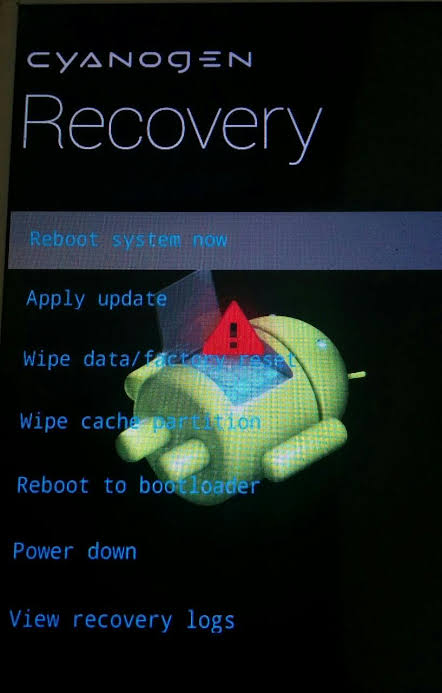
\includegraphics[width = 0.50\textwidth, center]{gfx/recovry.jpeg}    
    \caption{Recovery}
\end{figure}

\subsection{Recovery}
Recovery is an OS, which has a single purpose of allowing recovery. 
What it means is that it is a small OS which helps in fixing your main 
OS by providing tools to fix it ( Kind of like the live linux systems ). 
It is a minimal shell which allows for some fastboot and posix commands 
to run.\\\\It is most usefull in flashing zips which are either ROMs, 
custom kernels, or root binaries.The vanilla recovery that comes with 
the device does not allow for any such modifications, and this is where 
a custom recovery comes into picture. It allows for any modification 
and installation from within the recovery itself.

\subsubsection{Custom Recovery}
Custom recovery is the software which performs function of a recovery 
but allows for remote application i.e no need for another device to 
give commands to the system for it to work. One of the earlier custom 
recovery software was ClockworkMod which was one of the primary custom 
recovery for Android versions till 4.0, after which TWRP started to 
take over as the preferred recovery software.

\subsection{ADB and Fastboot}
ADB and Fastboot are utilities 

\subsubsection{Andoid Debugging Bridge}
Android Debugging Bridge ( known as ADB ) is a tool which allow for 
communication with an android device via USB. It is a shell with basic 
commands that allow a device to execute \textit{debug} commands. It is 
a basic version of a UNIX shell.

\begin{figure}
    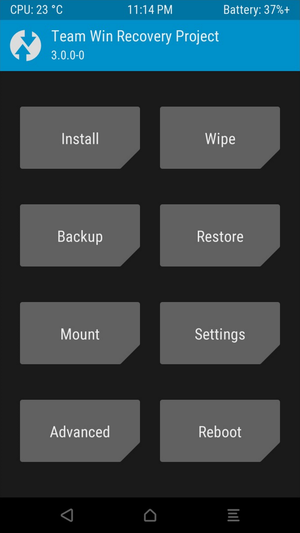
\includegraphics[width = 0.50\textwidth, center]{gfx/twrp.png}    
    \caption{TWRP}
\end{figure}


%%%%%%%%%%%%%%%%%%%%%%%%%%%%%%%%%%
\cleardoublepage

\bibliography{thesis}

%!TEX root = ../thesis.tex
% --------------------------
% Back matter
% --------------------------
%

\cleardoublepage

%\input{content/colophon}
% \cleardoublepage


\end{document}
